\chapter{Theoretical Foundations}
\label{chap:theoretical-foundations}
\section{Statistical Formulation of the Unfolding Problem}

Unfolding, also known as deconvolution, is the process of correcting detector distortions in experimental data to recover the true particle--level distributions.
%
This procedure is critical for comparing experimental results with theoretical predictions and for enabling detector--independent analyses.
%
The unfolding problem is inherently statistical and presents unique challenges due to its ill-posed nature.

\subsection{The Detector Response and Forward Problem}

The relationship between the particle--level truth distribution \(p(z)\) and the detector--level measured distribution \(p(x)\) is governed by the detector response function \(r(x|z)\), which encapsulates the resolution effects.\footnote{Efficiency and acceptance effects can also be incorporated if ``empty" events are allowed.}
\begin{equation}
    p(x) = \int r(x|z)\; p(z) \, \dd z.
\end{equation}
This equation describes the \textbf{forward problem}, where the true distribution \(p(z)\) is mapped to the measured distribution \(p(x)\).
%
The detector response function \(r(x|z)\) can often be estimated through detailed simulations.

\subsection{The Inverse Problem: Unfolding}

The goal of unfolding is to invert the forward problem and estimate truth, \(p(z)\) from data \(p(x)\).
%
Mathematically, this requires solving:
\begin{equation}
    p(z) = \int r^{-1}(z|x) \;p_{\text{measured}}(x) \, \dd x,
\end{equation}
where \(r^{-1}(z|x)\) represents the inverse response kernel.
%
However, this inversion is ill--posed because small fluctuations in \(p(x)\) can lead to large variations in \(p(z)\).
%
Regularization techniques are therefore essential to stabilize the solution.

\subsection{Likelihood-Based Formulation}
    In practice, unfolding is performed using statistical inference methods.
    %
    Given a set of measured data \(\mathbf{X}_{i=1}^N\), the likelihood function for a proposed truth distribution \(p(z; \theta)\), parametrised by \(\theta\), is
    \begin{equation}
        \mathcal{L}(\theta; \mathbf{X}) = \prod_{i=1}^{N} p(x_i;\; \theta),
    \end{equation}
    where
    \begin{equation}
        p(x; \theta) = \int r(x|z) \;p(x; \theta) \, \dd z.
    \end{equation}
    Maximizing this likelihood yields an estimate of the parameters \(\theta\), which define the unfolded truth distribution.
    %
    Regularization can be incorporated into this framework by adding penalty terms to the likelihood or by constraining the parameter space.

    \subsection{Regularization Techniques}
        Regularization mitigates the instability of unfolding by imposing constraints on the solution.
        %
        Common approaches include Tikhonov Regularization~\cite{Karl2005RegularizationReconstruction}, in which one adds a penalty term proportional to the norm of the second derivative of \(p(z)\), enforcing smoothness, and iterative methods which gradually refine estimates of \(p(z)\), regularizing by stopping before convergence.
        %
        These techniques balance fidelity to the measured data (prior independence) with stability of the unfolded solution.

    \subsection{Challenges in High Dimensional Phase Spaces}
    \label{subsec:challenges-in-high-dimensional-phase-spaces}
        \subsubsection{Binned methods}
        \label{subsubsec:binned-methods}
            A significant challenge that traditional unfolding methods face is the \emph{curse of dimensionality}.
            %
            As the number of measured observables increases, the statistical power required to populate discrete bins grows exponentially, quickly overwhelming even the largest datasets collected at modern experiments.
    
            Consider a measurement involving just four kinematic variables: transverse momentum, pseudorapidity, azimuthal angle, and invariant mass.
            %
            With a modest 20 bins per dimension, the resulting joint histogram requires \(\num{1.6d5}\) bins. Most of these bins will contain zero events, creating a sparse matrix that renders traditional unfolding techniques numerically unstable.
            %
            The relative uncertainty can scales as
            \begin{equation}
            \label{eq:relative-uncertainty}
                \text{Relative uncertainty} \propto \frac{1}{\sqrt{N_{\text{events}}} \cdot \prod_{i=1}^d \Delta z_i},
            \end{equation}
            where \(\Delta z_i\) are bin widths.
            %
            This scaling relationship emerges directly from Poisson counting statistics applied to multi--dimensional histograms.
            %
            For any histogram bin containing \(N\) events, the statistical uncertainty follows the standard Poisson scaling \(\sigma\propto\sqrt{N}\), yielding a relative uncertainty of \(\nicefrac{1}{\sqrt{N}}\).
            %
            In a \(d-\)dimensional measurement with bin widths \(\Delta z_1, \Delta z_2, \dots, \Delta z_d\), each bin occupies a hyper-volume
            \[
                V = \prod_{i=1}^d\Delta z_i
            \]
            in the measurement space.
            %
            Assuming approximately uniform event density, the expected number of events in any given bin scales as
            \[
                N_{\text bin} \propto N_{\text events} \times \prod_{i=1}^d\Delta z_i.
            \]
            The relative uncertainty in the measured differential quantity therefore follows the scaling law in \cref{eq:relative-uncertainty}.
            %
            This relationship reveals why traditional binned methods become increasingly impractical as dimensionality increases: maintaining fixed statistical precision requires exponentially more data or exponentially coarser binning, both of which severely limit the measurement's resolving power.
            
            Beyond a point, \textit{response matrix}, \(\mathbf{R}\) becomes not just ill--conditioned but genuinely rank--deficient, as sufficiently many bins have not just few events in them, but rather no events in them at all.
            %
            Hence, entire swaths of phase space remain unmeasurable regardless of accumulated statistics.
    
            \emph{Binning artifacts} compound these statistical challenges through systematic information loss.
            %
            The process of discretising continuous distributions into finite bins introduces artificial boundaries  onto the underlying physics.
            
            This discretization becomes particularly pernicious when dealing with correlation structures that span multiple dimensions.
            %
            Real particle collisions generate complex kinematic relationships---the angular distribution of decay products correlates with their energies, jet substructure variables depend on the overall jet momentum, and detector response functions couple seemingly independent observables.
            %
            Binning destroys these correlations by requiring low dimensional projections.
            %
            For instance, in jet substructure measurements, the relationship between different substructure variables contains valuable information about the underlying physics that can be obscured by independent binning of each variable.
            %
            Moreover, many theoretical predictions in particle physics are at the level of statistical moments or other distribution properties rather than full differential spectra.
            %
            Traditional unfolding methods require first unfolding the full distribution and then calculating these properties, which can lead to reduced precision in the moment predictions.
    
            The computational burden grows even faster than the statistical requirements.
            %
            Matrix inversion algorithms scale as \(\mathcal O(N^3)\) with bin number, meaning that the aforementioned four--dimensional histogram with \(\num{1.6d5}\) bins requires approximately \(\mathcal{O}(\num{d16})\) floating point operations to invert.
            %
            More fundamentally, the \emph{null spaces} and \emph{degeneracies} that plague two dimensional unfolding become dramatically worse in higher dimensions, where multiple truth configurations can project to identical detector signatures along numerous measurement axes simultaneously, because high dimensional measurements create complex geometric relationships between true and observed phase spaces.

            In addition to these limitations, traditional binned approaches suffer from an additional systematic weakness;
            %
            the response matrix \(R\) depends on on numerous variables that are typically marginalized over in order to bin the data.
            %
            While conventional methods construct \(R\) based on a limited set of binned observables, the true detector response depends on a much richer set of event characteristics.
            %
            These include additional kinematic variables not captured in the chosen binning scheme, event level properties such as particle multiplicity and missing energy, detector conditions like instantaneous luminosity and pileup activity, and correlations with other particles produced in the same collision.
            %
            Traditional unfolding methods are effectively forced to assume that \(R\) remains constant when averaged over these marginalized variables, but this assumption is patently incorrect when the detector response varies systematically across different regions of this extended phase space.
            %
            For example, the energy resolution for jets may depend not only on the jet's transverse momentum and pseudorapidity, variables often chosen for binning, but also on the jet's substructure, the presence of nearby particles, and the overall event topology.
            %
            By marginalising over these features, binned methods introduce systematic biases that can propagate through the unfolding procedure and distort the final measurements in ways that are difficult to quantify or correct.

        \subsubsection{Unbinned methods}
        \emph{Unbinned approaches} emerge as a natural response to these challenges, operating directly on individual events rather than aggregated histogram counts.
        %
        These methods exploit the event level structure that binning destroys, preserving the full kinematic information and correlation patterns within each recorded data point.
        %
        Instead of discretizing phase space into predetermined categories, unbinned techniques allow the data itself to determine the relevant resolution scales and correlation structures.
        
        Rather than explicitly modelling the response function \(r(x|z)\), modern techniques like \textsc{OmniFold}~\cite{andreassen_omnifold_2020} employ iterative reweighting strategies that learn implicit mappings between truth and detector-level distributions.
        %
        These methods sidestep the curse of dimensionality by avoiding explicit probability density estimation, instead focusing on weight optimization that preserves marginal distributions while respecting the detector response.

        The computational complexity shifts from matrix algebra to optimization landscapes, that scale more favourably with dimensionality.
        %
        While traditional unfolding requires inverting matrices that grow exponentially with dimension, unbinned methods typically employ gradient--based optimization that scales polynomially.
        %
        This trade-off exchanges the well--understood numerical properties of linear algebra for the more complex but ultimately more scalable challenges of machine learning optimization.

        Yet this transition introduces new sensitivities to model and hyperparameter choices that traditional methods avoid.
        %
        The implicit effect of the learning dynamics make it crucial to understand how optimization biases influence the final results.
        %
        These considerations establish the foundation for exploring how modern machine learning approaches navigate these challenges while preserving the statistical rigour that particle physics demands.

\section{Forward and Inverse Problems in HEP}
    The measurement process in high-energy physics experiments inherently involves two complementary mathematical challenges: the forward problem of predicting detector responses from particle-level interactions, and the inverse problem of recovering true physics distributions from observed detector measurements. These twin challenges form the conceptual foundation for understanding detector effects and developing unfolding methodologies.

\subsection{Mathematical Formulation}

The relationship between particle--level truth distributions and detector--level observations is governed by the Fredholm integral equation of the first kind~\cite{fredholm_sur_1903}
\begin{equation}
    p(x) = \int r(x|z)\,p(z) \, \dd z + \epsilon(x),
\end{equation}
where \(p(z)\) represents the true particle--level distribution, \(r(x|z)\) is the detector response kernel encoding resolution effects and acceptance, \(p(x)\) is the observed detector-level distribution, and \(\epsilon(x)\) accounts for measurement noise~\cite{weinberg_elementary_1963}.
%
This equation encapsulates the \emph{forward problem} when predicting \(p(x)\) given \(p(z)\), and the \textit{inverse problem} when estimating \(p(z)\) from data \(p(x)\).

For discrete histogram representations, this becomes a matrix equation:
\begin{equation}
    \label{eq:forward-binned}
    \boldsymbol{\mu} = \mathbf{R}\boldsymbol{\nu} + \boldsymbol{\epsilon},
\end{equation}
where \(\boldsymbol{\nu}\) and \(\boldsymbol{\mu}\) are vectors of true and observed bin counts, respectively, and \(\mathbf{R}\) is the smearing matrix containing conditional probabilities \(R_{ij} = P(\text{observed bin } i | \text{true bin } j)\)~\cite{cms_collaboration_measurement_2011}.

    \subsection{Challenges in Inverse Problems}
        The inverse problem in HEP is fundamentally and intrinsically ill--posed.
        %
        The response kernel is non--injective, i.e. different true distributions can produce identical observed distributions after detector smearing~\cite{palumbo_convergence_2025, neumaier_solving_1998}.
        %
        Furthermore, the distributions are ill--conditioned; small measurement errors \(\boldsymbol{\epsilon}\) amplify into large fluctuations in unfolded solutions due to small singular values in \(\mathbf{R}\)~\cite{ChungA, fernandez-martinez_effect_2014, carpio_inverse_2008}.
        %
        These intrinsic challenges with inverse problems are compounded by the fact that modern analyses involve a large number of observables, making brute-force phase space discretization computationally prohibitive~\cite{arratia_optimizing_2022, gaponenko_practical_2020, chan_unbinned_2023}.

        These challenges necessitate regularization techniques that impose physical constraints on solutions, such as Tikhonov regularization or iteration cutoffs before convergence, described above.

    \subsection{HEP Specific Considerations}
        Three aspects particularly complicate unfolding in particle physics compared to other inverse problem domains.
        %
        First, the response matrix $\mathbf{R}$ is estimated from from detailed Monte Carlo simulations\footnote{e.g. \textsc{Pythia}~\cite{bierlich_comprehensive_2022} for hadronization, \textsc{Geant4}~\cite{allison_recent_2016} for detector physics} that encode complex, non-Gaussian systematic uncertainties through their modelling assumptions~\cite{bozson_unfolding_2018, schmitt_data_2017, blobel_unfolding_2011, Huang2025MachineTechnique}.

        Second, detector response models contain hundreds to thousands of correlated nuisance parameters—including jet energy scale, b--tagging efficiencies, and pile--up effects-—that must be profiled or marginalized alongside the unfolding procedure~\cite{zhu2024multidimensional, Dorigo2020DealingReview, cranmer_histfactory_2012, ke_recent_2023}.

        Finally, the discrete nature of particle counting combined with highly variable event rates across phase space creates a challenging statistical landscape where Poisson uncertainties dominate in tails and signal regions, while Gaussian approximations may be valid elsewhere~\cite{kuusela_shape-constrained_2017, conrad_including_2003, giovanni_multi-dimensional_2010, from_new_2020}.

        A representative unfolding example is differential jet substructure measurements, where detector effects smear the true distribution of observables like jet mass or \(N-\)subjettiness.
        %
        The forward problem involves simulating jets through hadronization models and detector response, producing a migration matrix that relates true and reconstructed substructure observables.
        %
        The inverse problem requires unfolding these observables from reconstructed jets while accounting for correlated uncertainties in jet energy scale, angular resolution, and pile-up contamination~\cite{zardoshti_investigating_2017}.

        Similar challenges arise in unfolding differential cross sections as functions of transverse momentum, rapidity, or invariant mass, where detector acceptance and resolution vary significantly across the measurement range~\cite{gardi_statistics_2015}.
\section{Historical development: From matrix inversion to modern approaches}
\label{sec:ill-posed}
    The problem of unfolding has a rich history in high energy physics, with methods evolving alongside computational capabilities and statistical sophistication.
    %
    Early approaches relied primarily on simple correction factors applied to individual bins of histograms, appropriate only when detector effects were minimal.

    As measurements became more precise, regularised matrix inversion techniques emerged as the standard approach.
    %
    These methods discretise both the particle--level and detector--level distributions into bins, relating them through a response matrix \(\mathbf{R}_{ij}\) that describes the probability for an event in particle--level bin \(j\) to be observed in detector--level bin \(i\).
    %
    In component form, \cref{eq:forward-binned} can be written as
    \begin{equation}
        \mu_i = \sum_j R_{ij} \nu_{j},
    \end{equation}

    where \(\mu_{i}\) is the expected number of counts in detector--level bin \(i\) and \(\nu_{j}\) is the expected number of events in particle--level bin $j$.
    %
    Naively, one might attempt to solve this system by simply inverting the response matrix:
    \begin{equation}
        \nu_j = \sum_i (R^{-1})_{ji} \mu_i
    \end{equation}
    However, this direct inversion leads to wildly oscillating solutions with large variances---a manifestation of the ill-posed nature of the unfolding problem.
    %
    Additionally, \(R\) need not, and often is not, a square matrix.
    %
    To address this issue, a series of techniques were developed to invert \cref{eq:forward-binned} by imposing additional constraints.
    \begin{itemize}
    \item \textbf{Iterative Bayesian unfolding}~\cite{richardson_bayesian-based_1972, lucy_iterative_1974, Schmitt2017DataPhysics}: (also known as Lucy--Richardson deconvolution). Uses Bayes' theorem to iteratively update the estimate of the true distribution, with the number of iterations controlling regularization strength.
    \item \textbf{SVD unfolding}~\cite{hocker_svd_1996}: Applies singular value decomposition to the response matrix and suppresses contributions from small singular values that amplify statistical fluctuations.
    \item \textbf{TUnfold}~\cite{schmitt_tunfold_2012}: Formulates unfolding as a least-squares problem with Tikhonov regularization to penalize large second derivatives, preserving smoothness.
    \end{itemize}

These methods have served the field well for decades, particularly for one--dimensional measurements where binning is manageable.
%
However, they all share the common limitation of requiring discretization of the underlying distributions, which becomes increasingly problematic as measurements probe higher--dimensional spaces and more complex observables.


\section{Traditional unfolding methods in experimental analyses.}
\label{sec:binned-methods}
Traditional unfolding methods form the bedrock of detector corrections in high-energy physics (HEP), balancing statistical rigour with computational practicality.
%
This section provides an overview of established techniques, their mathematical foundations, implementation nuances, and limitations.

\subsection{Bin by bin correction.}  
The simplest unfolding approach applies multiplicative correction factors to observed bin counts:  
\begin{equation}
    \hat{\nu}_j = \frac{\mu_j - b_j}{C_j}, \quad C_j = \frac{\nu^{\text{MC}}_j}{\mu^{\text{MC}}_j},
\end{equation}  
where \(\mu_j\) is the observed count in bin \(j\), \(b_j\) the estimated background, and \(C_j\) the correction factor derived from Monte Carlo (MC) simulations relating particle--level generated (\(\nu^{\text{MC}}_j\)) and detector--level simulated (\(\mu^{\mathrm{MC}}_j\)) events~\cite{cowan_statistics_2021}. 

This method has the advantage of being computationally trivial, with no bin--to--bin correlations.
%
However, it fails to account for a non--diagonal response matrix (\(\exists i \neq j: \mathbf{R}_{ij} \ne 0)\).
%
This is illustrated most dramatically by the observation that biases persist even with \(C_j \rightarrow 1\) due to ignored cross--bin migrations~\cite{cowan_topics_2010}.

Used primarily in early LHC analyses\footnote{e.g., ATLAS~\cite{aad_measurement_2011, noauthor_implications_nodate} jet cross-sections}, bin--by--bin correction remains viable only for coarse binnings with negligible migration (\(<5\%\)~\cite{cms_collaboration_measurement_2011}) between adjacent bins.

\subsection{Matrix Inversion}  
When \(n_{\text{bins, truth}} = n_{\text{bins, reco}}\), the response matrix $\mathbf{R}$ is square.
%
Formally one can write an unfolded solution as  
\begin{equation}
    \hat{\boldsymbol{\nu}} = \mathbf{R}^{-1}\vb*{\mu},
\end{equation}  
and even propagate the covariance as  
\begin{equation}
    V_{\hat{\boldsymbol{\nu}}} = \mathbf{R}^{-1} V_{\vb*{\mu}} (\mathbf{R}^{-1})^T.
\end{equation}  
However, in practice, direct inversion is highly pathological.
%
This pathology can be quantified by the condition number
\begin{equation}
    \kappa(R\inv) = \frac{|\lambda_{\mathrm{max}}(R\inv)|}{|\lambda_{\mathrm{min}}(R\inv)|} \sim 10^3 - 10^6
\end{equation}
where $\lambda_{\mathrm{max}}(R\inv)$ and $\lambda_{\mathrm{min}}(R\inv)$ are the largest and smallest eigenvalues of $R\inv$ respectively.
%
The condition number measures how much a perturbation in the measured counts $\delta\mu$ perturbs the predicted truth counts $\delta\nu$.
%
The large condition number amplifies statistical fluctuations~\cite{belsley_regression_2005, pesaran_time_2015}.
%
Further, unphysical solutions such as negative bin count values can arise from noise--dominated eigenvectors.

Methods have been suggested to control this variance, such as Truncated SVD~\cite{deng_fast_2024}, involving discard singular values \(\sigma_i < \lambda_{\text{cut}}\)~\cite{TruncatedSVDDocumentation}, and Wiener-SVD~\cite{tang_data_2017}, a frequency--domain filtering method to maximize signal--to--noise ratio~\cite{zaroubi_wiener_1995}.
%
Despite this, matrix inversion's instability limits its utility.

\subsection{Iterative Bayesian unfolding}
Bayesian methods regularize through prior distributions \(p(z)\), yielding posterior estimates:  
\begin{equation}
    p({z}|{x}) \propto \mathcal{L}({x}|{z})p({z})
\end{equation}  
Common priors include uniform priors, entropy maximization \(p(z) \propto \exp(-\sum z_j \log z_j)\)~\cite{maeda_new_2013} and Gaussian processes enforcing smoothness~\cite{bozson_unfolding_2018}.
%
These provide natural uncertainty quantification but suffer from high computational cost, scaling poorly with dimensionality~\cite{cowan_bayesian_2007},sensitivity to prior misspecification, especially in low-statistics regions~\cite{cowan_bayesian_2006}, and difficulty interpreting credible intervals as frequentist coverage~\cite{james_statistics_2004}.

IBU, also known as Lucy Richardson deconvolution or D'Agostini iterative unfolding~\cite{dagostini_improved_2010} is an expectation maximization (EM) algorithm iteratively updates truth estimates
\begin{equation}
    \nu_j^{(k+1)} = \nu_j^{(k)} \sum_{i=1}^{N_{\text{Data}}} \frac{R_{ij}\; \mu_i}{\sum_{l=1}^{N_{\text{Truth}}} R_{il} \;\nu_l^{(k)}}
\end{equation}  

This method regularises via early stopping, by terminating at \(k \sim 4-6\) iterations before noise amplification~\cite{fish_blind_1995, shepp_maximum_1982}.
%
The initial guess \(\boldsymbol{\nu}^{(0)}\) biases the solution.
%
Some common choices include Generation \(\boldsymbol{\nu}_{\text{MC}}\), a uniform distribution, and data driven backwards folding \(\mathbf{R}^T \vb*{\mu}\).

 While computationally efficient, this approach lacks objective stopping criteria, requiring heuristic cross--validation~\cite{cowan_survey_2002} and underestimates uncertainties due to ignored iteration dependent covariance~\cite{cowan_statistical_1998}.

IBU is dominant in LHC analyses\footnote{e.g. differential jet substructure measurements~\cite{atlas_collaboration_measurement_2024}} because it balances simplicity with moderate-dimensional phase spaces (\(N_{\text{Truth}} \leq 20\)).

\subsection{Tikhonov Regularization}  
Tikhonov regularization is a penalized least--squares minimization method
\begin{equation}
    \hat{\boldsymbol{\nu}} =\underset{\boldsymbol{\nu}}{\arg\min} \left[ ||\vb*{\mu} - \mathbf{R}\boldsymbol{\nu}||^2 + \lambda ||\mathbf{L}(\boldsymbol{\nu} - \boldsymbol{\nu}_0)||^2 \right]
\end{equation}  
where \(\mathbf{L}\) is typically the discrete curvature operator\footnote{e.g. discrete second derivatives} and \(\boldsymbol{\mu}_0\) a prior estimate~\cite{cowan_topics_2009} that anchors solutions to MC predictions.
%
L-curve optimization balances the residual norm against the solution norm to choose \(\lambda\)~\cite{cowan_highlights_2011}.
%
The choice of \(\lambda\) sets the bias variance trade-off.
%
\(\lambda \rightarrow 0\) represents the high variance, low bias limit and \(\lambda \rightarrow \infty (\implies \hat{\boldsymbol{\nu}} \rightarrow \boldsymbol{\nu}_0)\) represents the low variance, high bias limit.
%
This method is implemented through the TUnfold package, which also provides automated \(\lambda\) tuning via global correlation minimization~\cite{schmitt_tunfold_2012}.
%
However this method struggles with non-differentiable features like threshold effects due to biased curvature penalties, and require ad hoc \(\lambda\) selection via L--curve curvature maximization.

\begin{note}{The RooUnfold package~\cite{adye_unfolding_2011} provides implemetations of bin--bin--bin corrections, matrix inversion, IBU, SVD, and TUnfold.}
\end{note}
\subsection{Template Fitting}  
Template fitting is a method suitable in cases where \(N_{\text{Data}} \gg N_{\text{Truth}}\).
%
In this case, one can construct detector--level templates for each truth bin:  
\begin{equation}
    \mu_i = \sum_{j=1}^{N_{\text{Truth}}} R_{ij} \nu_j + b_i
\end{equation}  
with \(\chi^2\) minimization:  
\begin{equation}
    \chi^2 = \sum_{i=1}^{N_{\text{Data}}} \frac{(\mu_i - \sum_j R_{ij}\nu_j - b_i)^2}{\sigma_i^2}
\end{equation}  

The solution then is overconstrained, since we leverage \(N_{\text{Data}}/N_{\text{Truth}} \sim 2-3\) for stability~\cite{britzger_linear_2022}.
%
Nuisance parameters are systematically modelled via template morphing~\cite{baak_interpolation_2015}.
%
Template fitting requires dense detector-level binning, which inflates statistical uncertainties. Template fitting is commonly used in Higgs coupling measurements where broad mass resolutions necessitate wide truth bins.
\subsection{Regularized Poisson Likelihood}  
For low-statistics regions, \cite{gaponenko_practical_2020} advocates minimizing
\begin{equation}
     -\log \mathcal{L}(x\,|\,z) + \lambda S(z)
\end{equation}  
\(S(z)\) penalizes non monotonicity in sharply falling spectra.
%
Using cubic B--splines with entropy regularization, this method avoids binning artifacts through continuous representations~\cite{gaponenko_practical_2020}.
%
However, it requires careful basis function placement to prevent endpoint spikes~\cite{fan_analysis_2022} and demands specialized optimization protocols (e.g., cooling schedules for \(\lambda\)~\cite{jia_sparse_2019}).

    \subsection{Summary}  
        \begin{table}
    \centering
    \begin{tabular}{lccc}
        \hline
        Method & MC dependence & Uncertainty propagation \\
        \hline
        Bin--by--bin & Extreme & Underestimated \\
        Matrix inversion & None & Exact but unstable \\
        IBU  & Moderate & Partial \\
        Tikhonov & Moderate & Full \\
        Template fit & Low & Full \\
        {Regularised Poisson}& Moderate & Full\\
        \hline
    \end{tabular}
    \caption{Comparing the MC dependence and uncertainty propagation of traditional unfolding methods.}
    \label{tab:binned-comp}
\end{table}


        Tab.~\ref{tab:binned-comp} summarizes the strengths and limitations of the methods discussed above.
        %
        These limitations motivated the use of machine learning in unfolding, a transition explored in subsequent sections.
        %
        However, traditional methods remain indispensable for validation and low--dimensional precision measurements where interpretability is crucial.
        
        \subsection{Regularization: Need, Approaches, and Limitations}
        The inherent ill--posedness of unfolding necessitates regularization to stabilize solutions against statistical fluctuations while preserving physical meaning.
        %
        This section systematically examines the theoretical justification for regularization, surveys dominant methodologies, and critically evaluates their limitations in high energy physics applications.
        
        \subsubsection{The Necessity of Regularization}  
         As discussed earlier, unfolding inverse problems in HEP exhibit pathological characteristics that demand regularization.
        %
        Regularization counteracts these issues by introducing prior knowledge about \(p(z)\), typically favouring smoothness or similarity to Monte Carlo (MC) predictions.
        %
        However, as Zech and Bohm emphasise in~\cite{Bohm2025IntroductionPhysicists}, this unavoidably discards information---regularized solutions cannot resolve features finer than the detector resolution or distinguish theories predicting distributions within the regularization bias.
        
        Early termination (typically \(k \sim 4-6\)) acts as implicit regularization by preventing overfitting~\cite{multhei_iterative_1987}.

    \subsubsection{Limitations and practical challenges}  
        \paragraph{Subjectivity-objectivity trade-off}  
            All regularization methods inject subjective choices---smoothness scales, prior distributions, stopping criteria and so on—--that bias results.
            %
            This trade--off reveals a deeper epistemological issue: regularization transforms the question from ``what does the data show?" to ``what does the data show given our assumptions about smoothness?"
            %
            While Zech~\cite{zech_regularization_2011} and Kuusela~\cite{kuusela_uncertainty_2016} argue for publishing unregularized results alongside regularized ones, this approach, though transparent, may be insufficient.
            %
            The unregularized results often contain artifacts that obscure physical interpretation, and a well chosen regularization scheme can eliminate solutions that are patently unphysical.
            
            A more nuanced approach would involve explicitly testing regularization assumptions against physical models where possible, and developing domain--specific regularization schemes that incorporate known physical constraints rather than generic smoothness priors.
            %
            This would shift the subjectivity from mathematical convenience to physics--informed choices, making the trade--offs more scientifically meaningful rather than purely computational.

        \paragraph{High dimensional regimes}  
            Traditional methods fail catastrophically in \(d \gtrsim 4\) phase spaces for multiple reasons.
            %
            Binned approaches require \(n^d\) histogram bins struggling to effectively sample an increasingly sparse phase space, are shown in \cref{subsubsec:binned-methods}.
            %
            Global smoothness assumptions become untenable for multi--scale features~\cite{fernandez-martinez_curse_2020, xia_bayesian_2022, hocker_svd_1996} straining regularization methods that rely on them. 

            As the number of dimensions increases, the binning also increasingly distorts error propagation. 
            %
            Bayesian credible intervals can exhibit poor frequentist coverage, as shown Fig. 4 of~\cite{Zhang2006AIntervals},~\cite{eberly_estimating_2003, szabo_frequentist_2015}, and correlated systematic uncertainties\footnote{e.g., jet energy scale} introduce non--convex likelihoods~\cite{berger_simplified_2023, Berger2017LectureATLAS}.

        \paragraph{Spectrum dependent biases}  
            Sharply falling spectra\footnote{e.g., proton momentum in~\cite{arnison_transverse_1982}} exacerbate regularization artifacts~\cite{gaponenko_practical_2020}.
            %
            Entropic priors overweight high\(-z\) regions, distorting tails~\cite{caticha_entropic_2004, rodriguez_entropic_2002, Handley2019Maximum-EntropyDistribution, brewer_entropic_2009},
            %
            finite sample sizes truncate measurable phase space, creating cutoff--induced spikes~\cite{finotello_functional_2025, marchand_bayesian_2012},
            %
            and curvature penalties conflict with natural spectral shapes, requiring physics--informed regularization strategies~\cite{lee_explicit_2023, moosavi-dezfooli_robustness_2018, zech_analysis_2016, Baron2020ExtendingMethod}.  

        Recent advances aim to mitigate these limitations in various ways.
        %
        For example, adversarial regularization involves training discriminators to enforce physical consistency rather than explicit smoothness\~cite{Terjek2019AdversarialRegularization}.
        %
        Differentiable unfolding methods embed detector response in neural networks enabling gradient--based \(\lambda\) optimization~\cite{delaRosa2020DifferentiableAnalysis}.
        %
        However, no universal solution exists.
        %
        The choice of regularization must align with analysis--specific priorities,
        %
        As detector granularity increases, developing dimension--agnostic regularization schemes remains an open challenge requiring collaboration between statisticians and physicists.
\section{Unbinned Methods: Statistical Considerations}  
    The evolution from binned to unbinned unfolding methodologies represents a paradigm shift in high--energy physics, driven by the need to preserve fine--grained kinematic information while managing the statistical and computational complexities of high-dimensional phase spaces.
    %
    This section systematically analyses the theoretical foundations, practical challenges, and performance trade-offs that this transition entails.
    \subsection{Principles and Implementations}
        The unbinned approach to unfolding represents a fundamental shift from traditional histogram--based methods.
        %
        Rather than discretising data into bins, unbinned unfolding preserves the complete kinematic information by operating directly on individual event tuples \(\{(z_1, x_1), ..., (z_N, x_N)\}\) where each \(z_i\) represents a particle--level event and \(x_i\) its corresponding detector--level measurement.
        %
        This approach eliminates information loss from binning and naturally handles high--dimensional phase spaces where binning becomes prohibitive.

        The central goal of one class of unbinned unfolding methods is to estimate a reweighting function \(w(z)\) that transforms the particle--level Monte Carlo distribution, referred to as \emph{generation} (Gen.) to match the underlying truth that was forward folded into the data.
        %
        Formally, this function satisfies:
        \begin{equation}
            p(z) = w(z) \cdot q(z),
        \end{equation}
        where \(q(z)\) is the distribution of the generation.

        Modern unbinned methods leverage machine learning techniques, particularly those designed for density (ratio) estimation.
        %
        These approaches fall into two main categories: reweighting methods and direct generative modelling.
        \subsubsection{Reweighting Methods}
            The most established approach in this category is \textsc{OmniFold}, which employs an iterative procedure inspired by the Iterative Bayesian Unfolding (IBU) algorithm.
            %
            \textsc{OmniFold} alternates between two steps that estimate likelihood ratios using binary classifiers.
            
            In each iteration \(k\), \textsc{OmniFold} first trains a classifier to distinguish between data and simulated detector--level events, referred to as \emph{simulation} (Sim.), yielding the ratio
            \begin{equation}
                \nu^{(k)}(x) = \frac{p(x)}{q^{(k)}(x)},
            \end{equation}
            where \(q^{(k)}(x)\) represents the distribution from simulation weighted by the current iteration's particle--level weights.

            This detector--level ratio is then propagated back to particle level through the Monte Carlo pairing.
            %
            For each generation event \(z_i\) with corresponding simulation event \(x_i\), the weight update follows:
            \begin{equation}
                w^{(k+1)}(z_i) = w^{(k)}(z_i) \cdot \nu^{(k)}(x_i).
            \end{equation}
            The process, in principle, continues until convergence, at which point the final weights \(w(z)\) provide the desired transformation from generation to truth.
            %
            This connection to likelihood ratio estimation can be explicitly proven---for a binary cross entropy optimized classifier \(f\), the likelihood ratio between the distributions it classifies is
            \[
                LR = \frac{f}{1-f}
            \]
        \subsubsection{Generative Modeling}
            An alternative approach employs generative models to directly learn the conditional distribution \(p(z|x)\).
            %
            Among these, Conditional Invertible Neural Networks (cINNs)~\cite{AnanthaPadmanabha2021SolvingNetworks} offer a particularly elegant framework.
            
            cINNs learn a diffeomorphic mapping \[g_\theta: {Z} \to {X}\] between particle and detector levels, parameterized by neural network weights \(\theta\).
            %
            The invertibility constraint ensures that for any detector--level observation \(x\), we can directly sample the corresponding particle--level distribution through the inverse mapping.
            %
            The key advantage lies in the tractable Jacobian computation:
            \begin{equation}
                p(z|x) = p(x|z) \frac{p(z)}{p(x)} = \left|\det \frac{\partial g_\theta}{\partial z}\right|^{-1} p(g_\theta^{-1}(x)|x),
            \end{equation}
            enabling direct sampling from the posterior \(p(z|x)\) without iterative procedures~\cite{Bellagente2020InvertibleAgain}.

            Generative models, due to the much greater expressiveness that is necessary for them to model the functional representations needed, are succeptible to training challenges such as mode collapse\footnote{Normalizing flows however, due to the structural constraints that invertibility imposes, are resistant to mode collapse.}.
            %
            Ensuring stable convergence of generative models can get increasingly difficult for high-dimensional problems.
            
            More recently, Schrödinger Bridge Unfolding~\cite{Butter2025GenerativeMapping} has emerged as a method that frames unfolding as an optimal transport problem.
            %
            This approach minimizes the Kullback--Leibler divergence between joint distributions while constraining the marginal to match observed data:
            \begin{equation}
                \inf_{p(z,x)} D_{\text{KL}}\Big(p(z,x) \parallel p_{\text{MC}}(z,x)\Big) \text{ subject to } p(x) = p_{\text{Data}}(x).
            \end{equation}
            This formulation provides theoretical guarantees on the uniqueness of the solution and offers improved stability compared to purely generative approaches.
        \subsection{Statistical Considerations in Unbinned Regimes}  
            Neural networks implicitly regularize via inductive controls. 
            %
            e.g., convolutional layers enforce translational symmetry in jet images~\cite{Kheddar2025ImageSurvey}.
            %
            However, this introduces model--dependent smoothing scales requiring careful validation against closure tests~\cite{Cowan2011AsymptoticPhysics}.

            Reweighting based methods can propagate one part of the overall uncertainty through event weights.
            \begin{equation}
                \text{Cov}[O] = \sum_{i=1}^N w_i^2 O(z_i)^2 - \left(\sum_{i=1}^N w_i O(z_i)\right)^2,
            \end{equation}
            for observable \(O(z)\)~\cite{LHCHiggsCrossSectionWorkingGroup2012HandbookDistributions}.
            %
            While avoiding binning--induced correlations, unbinned inference requires re--conceptualizing what the unbinned equivalent of the covariance matrix would be in order to appropriately account for correlations in the unfolded data.
    \subsection{Limitations in Complex Phase Spaces}  
        \subsubsection{Model Misspecification}  
            Generative models assume that \[q(z) > 0 \implies p(z) > 0,\] meaning that wherever generation (particle--level Monte Carlo) assigns positive probability density, \(q(z) > 0\), the true distribution also has positive probability density, \(p(z) > 0\).
            %
            This assumption ensures that the generative model does not learn to generate events in regions of phase space where the true physics has zero probability.
            %
            It is fundamental to the validity of generative unfolding approaches such as conditional Invertible Neural Networks (cINNs) and Variational Autoencoders (VAEs)~\cite{Shmakov2025FullDiffusion}.
            %
            Generative models learn to map from detector--level measurements to particle--level distributions by generating samples from the learned posterior.
            %
            If the generation samples in kinematically forbidden regions or unphysical phase space, the unfolded results will include spurious events that contaminate the measurement.
            %
            The assumption requires that the generative model be properly constrained to respect the physical boundaries of the true distribution.
            
            Violations of this assumption can occur when generative models, trained on imperfect or limited data, learn to extrapolate beyond the true physical support and generate samples in unphysical regions.
            %
            This is particularly problematic given the tendency of neural networks to produce overconfident predictions in regions with sparse training data.
            
            Conversely though, enforcing this support containment requirement has practical implications for unfolding performance.
            %
            Since the generative model can only learn to assign meaningful probability density to regions of phase space adequately represented in the training data, kinematic regimes that are poorly sampled or entirely absent from the Monte Carlo generation are rendered effectively invisible to the unfolding procedure regardless of their importance in the truth distribution.
            %
            This limitation becomes particularly concerning for new physics searches, where signatures may manifest in previously unexplored regions of phase space.
            %
            Novel phenomena occurring outside the support of the generative model where cannot be properly unfolded and may remain undetected~\cite{Amsler2008MonteTechniques}. 
            
            The assumption thus places stringent requirements on Monte Carlo coverage and highlights the importance of comprehensive phase space sampling in training data preparation for generative unfolding methods.
            %
            Hybrid approaches combining discriminative and generative components show promise for anomaly detection~\cite{DiMattia2019ADetection, Terjek2019AdversarialRegularization}.
\section{Evaluation metrics for unfolding.}
    The evaluation of unfolding methods presents unique challenges due to the ill--posed nature of the inverse problem.
    %
    While the goal of unfolding is conceptually straightforward, to recover the true particle--level distribution from detector--level observations, quantifying the success of this recovery requires careful consideration when the downstream use of the data is unknown.
    %
    Task--specific evaluation becomes more tractable when clear physics objectives are defined.
    %
    For example, when unfolding is performed to measure a specific parameter such as \(\alpha_S\), evaluation metrics can be designed to directly assess how well the unfolding procedure enables accurate parameter extraction.
    %
    This section focuses on metrics and approaches for evaluating unfolding performance, considering both traditional binned techniques and modern unbinned methods, for general--purpose unfolding applications where the downstream use is not known.
    %
    Metrics for assessing accuracy, precision, and uncertainty quantification are assessed and practical considerations for their application in high energy physics analyses are discussed.

    
    \subsection{Statistical metrics for evaluating point estimates.}
        \subsubsection{Residual based metrics.}
            The most intuitive approach to evaluating an unfolding method is to compare the unfolded distribution to the true distribution when it is known\footnote{e.g., in simulation studies}.
            %
            Simple residual--based metrics quantify the difference between the estimated and true distributions.
            %
            For binned methods, the bin by bin residual is defined as:
            \begin{equation}
                \delta_i = \hat{t}_i - t_i
            \end{equation}
            where \(\hat{t}_i\) is the unfolded count in bin \(i\) and \(t_i\) is the true count.
            %
            Various summary statistics of these residuals can be computed, including
            \begin{align}
                \text{MSE} &= \frac{1}{n}\sum_{i=1}^{n}(\hat{t}_i - t_i)^2\\
                \text{RMSE} &= \sqrt{\frac{1}{n}\sum_{i=1}^{n}(\hat{t}_i - t_i)^2}\\
                \text{MAE} &= \frac{1}{n}\sum_{i=1}^{n}|\hat{t}_i - t_i|
            \end{align}
            The MSE might be preferred because it is easier to do calculus with, the RMSE preferred because it is expressed in the units of the original data rather than squared units, but they are manifestly functionally equivalent.
            %
            The choice between the MSE and MAE depends on the specific requirements of the analysis.
            %
            MSE more heavily penalizes large errors due to the squaring operation, making it more sensitive to outliers and extreme residuals.
            %
            MAE treats all errors equally regardless of magnitude and proves more robust to outliers, making it preferable when the unfolding procedure should not be dominated by a few problematic bins or events.
            %
            The square function though is more amenable to calculus than the absolute value function.
            %
            In high energy physics applications, RMSE is the most commonly used metric, while MAE may be provided as valuable complementary information.
            
            While these metrics are straightforward, they have limitations in the context of unfolding.
            %
            In particular, they treat all bins equally, even though certain regions of phase space may be physically more significant than others.
            %
            Additionally, these metrics do not account for the correlations between bins introduced by the unfolding process.
            
            For unbinned methods, where the output is a set of weights or a continuous probability density, these metrics must be adapted.
            %
            One approach is to bin the unbinned unfolded distributions and then apply the above metrics, though this introduces binning artifacts that the unbinned method was designed to avoid.

        \subsubsection{Distributional distance metrics.}
        \label{subsubsec:distributional-distance-metrics}
            Given the limitations of simple residual metrics, distributional distance measures provide a more comprehensive assessment of unfolding performance.
            %
            These metrics compare the entire unfolded distribution to the true distribution.

            The \emph{Kullback--Leibler (KL) divergence}~\cite{kullback_information_1951} measures the information lost when using the unfolded distribution to approximate the true distribution.
            
            \begin{equation}
            D_{\text{KL}}(p||q) = \int p(x) \log \frac{p(x)}{q(x)} \;\dd x,
            \end{equation}
            where \(p\) is the true distribution and
            \(q\) is the unfolded distribution.
            %
            While theoretically sound, KL divergence can be numerically unstable when the support of the distributions differs.
            
            The \emph{Vincze--Le Cam (VLC) divergence}~\cite{vincze_concept_1981,Cam1986AsymptoticTheory} is symmetric alternative to KL divergence that is both bounded and highly convex~\cite{melbourne_strongly_2020}.
            \begin{equation}
                \Delta(p, q) = \frac{1}{2}\int \frac{(p(\lambda) - q(\lambda))^2}{p(\lambda) + q(\lambda)} \;\dd\lambda.
            \end{equation}
            This metric is particularly useful for comparing unfolding methods as it provides a balanced assessment of differences across the entire distribution and has been used in comparative analyses of various unfolding approaches~\cite{andreassen_omnifold_2020, komiske_preserving_2021}.

            The \emph{Wasserstein metric}~\cite{L.N.VasersteinIssue3Pagesnobr6472/nobr}, also known as the \emph{Earth mover's distance},"~\cite{rubner_metric_1998} provides a measure of the minimum ``work" required to transform one distribution into another.
        \begin{equation}
            W_p(p, q) = \left(\inf_{\gamma \in \Gamma(p, q)} \int\int |x-y|^p d\gamma(x, y)\right)^{1/p},
        \end{equation}
        where \(\Gamma(p, q)\) is the set of all joint distributions with marginals \(p\) and \(q\).
        %
        This metric is particularly useful for unfolding evaluations as it accounts for both the magnitude and location of discrepancies between distributions.
        Table~\ref{tab:dist_metrics} summarizes the various distributional metrics and their relative strengths for unfolding evaluation.
        \begin{table}
\centering
\caption{Distributional distance metrics for unfolding evaluation}
\label{tab:dist_metrics}
\begin{tabular}{lcccc}
\hline
 & Symmetric & Bounded & Support sensitivity & Compute Cost \\
\hline
\(D_{\textrm{KL}}\) & No & No & High & Low \\
\(\Delta_{\textrm{VLC}}\) & Yes & Yes & Medium & Low \\
\(W_2\) & Yes & No & Low & High \\
\hline
\end{tabular}
\end{table}
        \subsection{Uncertainty quantification metrics}
        Beyond point estimates, properly evaluating unfolding methods requires assessing the accuracy of their uncertainty estimates. 
        %
        This is particularly important in particle physics, where uncertainties propagate to downstream analyses such as parameter fitting.
        \subsubsection{Pull distributions}
        \label{subsubsec:pull-distributions}
            Pull distributions offer a rigorous way to evaluate the calibration of reported uncertainties.
            %
            For a given unfolded bin or parameter \(\theta\), the pull is defined as
            \begin{equation}
                \text{Pull}\,{\theta} = \frac{\hat{\theta} - \theta_{\text{true}}}{\sigma_{\hat{\theta}}}
            \end{equation}
            where \(\hat{\theta}\) is the unfolded estimate, \(\theta_{\text{true}}\) is the true value, and \(\sigma_{\hat{\theta}}\) is the reported uncertainty.
            %
            For a well--calibrated method, the pull distribution across many pseudo--experiments should follow a standard normal distribution, \(\mathcal{N}(0,1)\).
            This follows from the definition of random variables.
            %
            Since the pull is defined as the ratio of the bias to the estimated uncertainty, for a properly calibrated unfolding method, two conditions must be satisfied simultaneously.
            %
            First, the method must be unbiased, meaning that across many pseudo experiments, the estimated values should equal the true values on average, resulting in zero mean for the numerator.
            %
            Second, the reported uncertainties must accurately reflect the actual variability of the estimates, such that the denominator correctly represents the standard deviation of the numerator.
            
            When both conditions are met, the pull becomes a standardized random variable.
            %
            For sufficiently large sample sizes, many unfolding estimators approach normality due to the Central Limit Theorem, since they often involve weighted sums or averages of many events.
            %
            When the underlying estimator is approximately normally distributed, if it satisfies the two conditions above that set its mean and standard deviation to \(0\) and \(1\) respectively, the population of sample pulls must be distributed as a standard normal.
            
            A pull distribution with non-zero mean indicates systematic bias in the unfolding procedure,
            %
            Deviations from unit standard deviation indicate either overestimation or underestimation of uncertainties.
            
            In the context of binned unfolding, pull distributions can be computed for each bin, while for unbinned methods, they can be applied to derived quantities or parameters of interest.
            %
            For Bayesian methods, pulls can be calculated using the mean and standard deviation of the posterior distribution~\cite{Knapik2012BayesianPriors}.
        \subsubsection{Coverage properties}
            Related to pulls but more direct is the evaluation of coverage properties of confidence or credible intervals.
            %
            For a nominal 68\% confidence interval, approximately 68\% of intervals computed across many pseudo-experiments should contain the true value.
            %
            Systematic deviations from nominal coverage indicate issues with the uncertainty estimation.
            %
            Coverage can be assessed through closure tests. These involve generating multiple datasets from a known truth, applying the unfolding procedure, and checking the fraction of times the true value falls within the reported confidence intervals.
            %
            Coverage plots plot the actual coverage versus the nominal coverage across different confidence levels.
            %
            The example in \cref{fig:coverage} shows expected coverage properties for two different unfolding methods, Tikhonov regularisation and IBU, as a function of the regularisation parameter.
            \begin{figure}
                \centering
                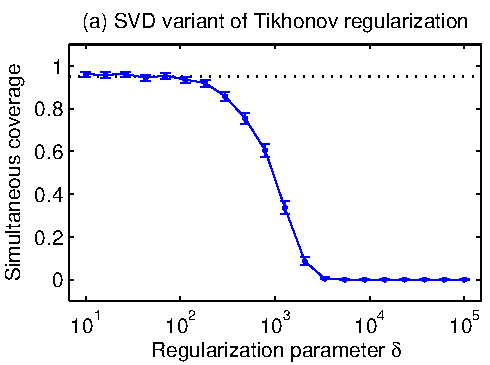
\includegraphics[width=0.5\linewidth]{figures/chapter-02/incJets_lumFactor150nBinsE30nBinsF30JointCoverageSVD.pdf}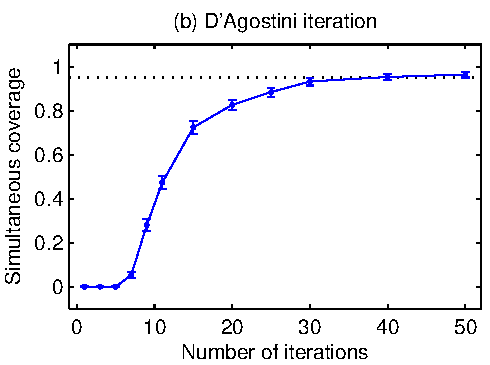
\includegraphics[width=0.5\linewidth]{figures/chapter-02/incJets_lumFactor150nBinsE30nBinsF30JointCoverageDAgostini.pdf}
                \caption[Coverage properties of Tikhonov regularisation and IBU]{Coverage of 95\% confidence intervals with Tikhonov regularisation (left) and IBU (right).
                %
                The error bars are given by the 95\% Clopper–Pearson intervals and the nominal confidence level is shown by the dotted line.
                %
                When the regularization is strong (fewer iterations in the case of IBU), both methods undercover substantially. IBU~\cite{kuusela_shape-constrained_2017}}
                \label{fig:coverage}
            \end{figure}
    \subsubsection{Variance and bias decomposition}
        The total error of an unfolding method can be decomposed into bias and variance components,
        \begin{equation}
        \text{MSE}(\hat{t}) = \text{Bias}^2(\hat{t}) + \text{Var}(\hat{t}),
        \end{equation}
        where \(\text{Bias}(\hat{t}) = \mathbb{E}[\hat{t}] - t\) and \(\text{Var}(\hat{t}) = \mathbb{E}[(\hat{t} - \mathbb{E}[\hat{t}])^2]\). 
        
        This decomposition is particularly valuable for understanding the trade--offs inherent in regularized unfolding methods, where stronger regularization typically reduces variance at the expense of increased bias.
        %
        Different applications might prioritize minimizing one component over the other, making this decomposition essential for method selection.

    \subsection{Evaluation of correlation structure}
        Traditional evaluation metrics often focus on marginal distributions, overlooking an important aspect of unfolding: the correlation structure between different bins or events.
        %
        Properly accounting for these correlations is crucial for downstream analyses.
        \subsubsection{Covariance Matrix Assessment}
            For binned methods, the full covariance matrix of the unfolded distribution provides information about bin--to--bin correlations.
            %
            A useful measure is the correlation matrix, defined as
            \begin{equation}
                \text{Corr}_{ij} = \frac{\text{Cov}_{ij}}{\sqrt{\text{Cov}_{ii}\text{Cov}_{jj}}}
            \end{equation}
            Comparing the correlation structure of the unfolded distribution to that of the true distribution (when known, e.g. in simulation studies) can reveal systematic distortions introduced by the unfolding procedure.
        \subsubsection{Event--to--event correlation metrics}
            For unbinned methods event--to--event correlations in the unfolded weights can significantly impact downstream inference.
            %
            These correlations can be quantified by studying the weight correlation as a function of distance.
            %
            For any pair of events, one can compute the correlation between their weights as a function of their distance in feature space.
            %
            One can also estimate the reduction in statistical power due to correlated weights
            \begin{equation}
                \label{eq:n-eff}
                N_{\text{eff}} = \frac{\left(\sum_{i} w_i\right)^2}{\sum_{i} w_i^2 + 2\sum_{i<j} w_i w_j \text{Corr}(w_i, w_j)}
            \end{equation}
            In this equation, \(N_{\text{eff}}\) represents the effective number of independent observations when event weights are correlated, derived from the variance properties of weighted sums.
            %
            The numerator, \(\qty(\sum w_i^2)\) represents the square of the total weighted sample size.
            %
            The denominator consists of two components, which together account for the increased variance introduced by weight correlations.
            %
            The first term, \(\sum w_i^2\), captures the variance contribution from individual event weights, similar to the standard effective sample size formula for independent weighted observations.
            %
            The second term, \(2\sum_{i<j} w_i w_j \operatorname{Corr}(w_i, w_j)\), accounts for the covariance contributions between all pairs of events, where the factor of 2 arises because each pair appears only once in the sum over \(i<j\).

            When weights are uncorrelated, \(\operatorname{Corr}(w_i, w_j) = 0,\) and the formula reduces to the familiar \(N_{\text{eff}}=\nicefrac{\qty(\sum w_i)^2}{\sum w_i^2}.\)
            %
            However, upon unfolding methods, nearby events in phase space often receive similar weight corrections\footnote{as will be discusseed in greater detail in \cref{chap:unbinned_correlations}}, leading to correlations that increase the denominator and reduce the effective sample size.
            %
            This reduction quantifies the loss of statistical power compared to an ideal scenario with independent weights.

            The formula emerges from considering the variance of weighted observables.
            %
            For a weighted sum, \(S = \sum w_i\,x_i\), the variance is
            \[
                \operatorname{Var}(S) = \sum_i \sum_j w_i w_j \operatorname{Cov}(x_i, x_j),
            \]
             which is the denominator of the \cref{eq:n-eff}.
             %
             The effective sample size is then defined as the ratio of the squared expectation to the variance, providing a measure of statistical efficiency that accounts for both weight magnitudes and their correlations.
             
            \cref{fig:corr-decay} illustrates how event correlations typically decay with distance, with the correlation length scale increasing with detector resolution effects.
            \begin{figure}
                \centering
                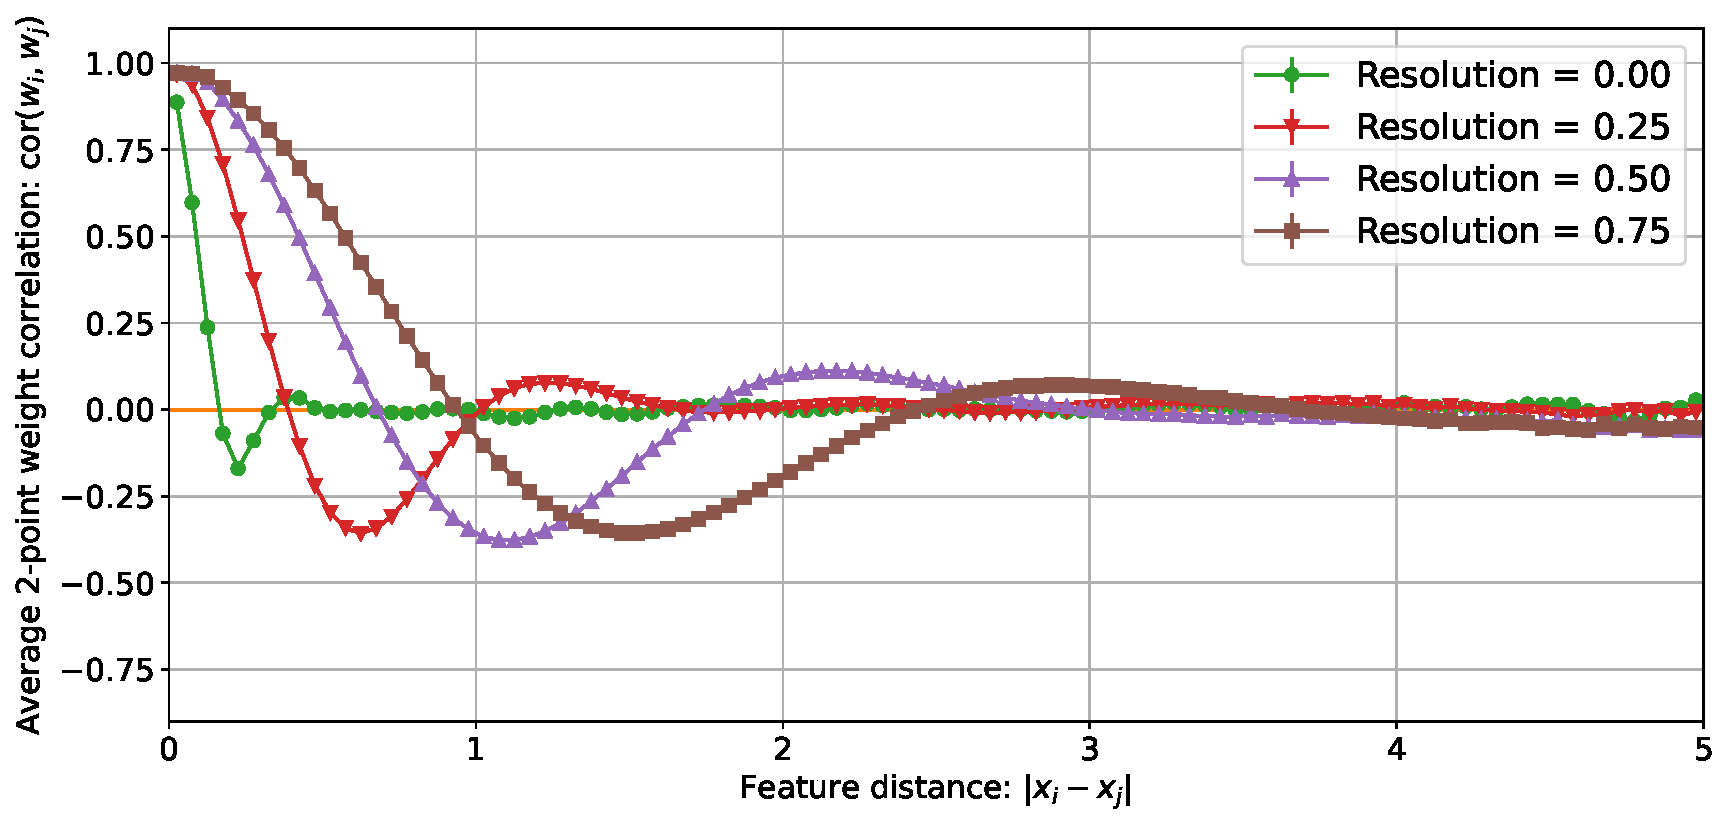
\includegraphics[width=\linewidth]{figures/chapter-02/weight-correlation-vs-distance-1d-set1.pdf}
                \caption[Weight correlation between event pairs as a function of distance between events.]{Average weight correlation between two events as a function of the absolute distance between the events in the observable for Gaussian data unfolded using \textsc{OmniFold}~\cite{Desai:2025mpy}.\protect\footnotemark
                }
                \label{fig:corr-decay}
            \end{figure}
            \footnotetext{Figure created by Owen Long}
    \subsection{Method specific evaluation metrics}
        \subsubsection{Iterative methods}
            For iterative methods like Iterative Bayesian Unfolding (IBU) or \textsc{OmniFold}, convergence behaviour provides important diagnostic information.
        %
        To study the convergence behaviour, we plot metric values (e.g., \(\chi^2\) or NLL) as a function of iteration number.
        %
        We then compare unfolded distributions at different iterations to assess stability and analyse how the bias--variance trade off evolves with iteration number.

        \subsubsection{Bayesian Methods}
            For Bayesian unfolding methods such as Fully Bayesian Unfolding (FBU)~\cite{choudalakis_fully_2012} or \textsc{Neural Posterior Unfolding} (NPU)~\cite{acosta2024npu}, additional posterior specific metrics are relevant.
            %
            We can compare detector level data to detector level predictions generated from the posterior.
            %
            We assess convergence using standard MCMC based diagnostics like Gelman--Rubin statistics or effective sample size.
            %
            The width of the posterior allows us to evaluate the posterior uncertainty in relation to the true frequentist variance.

    \subsection{Practical considerations.}
        In general, when comparing different unfolding methods, a structured evaluation framework ensures fair and comprehensive assessment. Such a framework should consider
        \begin{itemize}
            \item Computational efficiency: Measure training time, inference time, and memory requirements.
            \item Dimensionality scaling: Assess how performance metrics change as the dimensionality of the problem increases.
            \item Prior dependence: Evaluate robustness to different initial simulations.
            \item Regularisation parameter sensitivity: Compare how performance varies with changes in regularization strength.
        \end{itemize}

        In real experimental settings where the truth is unknown, evaluation presents additional challenges that require alternative pragmatic approaches.
        %
        For example, when the true distribution is unavailable, data-splitting techniques can provide useful validation.
        %
        The two most commonly used techniques are cross-validation, where we split the detector--level data, unfold one portion, then refold it, and compare predictions against the held--out portion; and bootstrapping where we generate multiple resampled datasets to assess the stability of the unfolding procedure.

        Closure tests involve applying the full analysis chain (forward model followed by unfolding) to a known input distribution.
        %
        While not a direct evaluation of performance on real data, closure tests provide confidence in the methodology.
        %
        The simplest kinds of closure tests involve apply detector simulation to a known particle--level distribution, then unfolding the resulting detector--level distribution and compare with the original input.
        %
        This procedure can then be modified by using a different particle-level input than the one used to train the unfolding method, testing robustness to prior misspecification.
        
        Evaluating how unfolding methods propagate systematic uncertainties is crucial for real-world applications.
        %
        We can test the sensitivity of the method to systematic uncertainties by applying variations to the response matrix based on known systematic uncertainties and assessing the impact on unfolded distributions.
        %
        For methods that support nuisance parameter profiling, evaluating how effectively nuisance parameters are profiled out is a gold standard test for the effectiveness of the method.
        
        Rigorous evaluation of unfolding methods requires a multi--faceted approach that considers accuracy, uncertainty quantification, and computational performance.
        %
        The metrics and frameworks presented in this section provide a comprehensive foundation for assessing both traditional and machine learning-based unfolding techniques.
        %
        For binned methods, established metrics like \(\chi^2\) and coverage tests remain valuable, while for unbinned approaches, distributional metrics like Wasserstein distance and VLC divergence offer more appropriate evaluation.
        %
        Regardless of the method, uncertainty calibration through pull distributions and correlation structure assessment are important to validate any measurement.
        %
        As unfolding methods continue to evolve, particularly with the advent of machine learning approaches, evaluation metrics must adapt accordingly.
        %
        The framework presented here is designed to be extensible, accommodating new methods and application domains while maintaining rigour and comparability